\section{Implementierung und Durchführung der Prototypen}
\label{ch:implementierung}

Dieses Kapitel stellt die praktische Testumgebung, die ausgeführten Testszenarien sowie den technischen und syntaktischen Vergleich zwischen Selenium und Cypress dar. Die Ausformulierung stellt dabei konkrete Projektbezüge zur Webanwendung Puma bei der JUMO GmbH \& Co. KG her.

\subsection{Testumgebung und Rahmenbedingungen}
\label{sec:testumgebung}

Die Tests wurden im betrieblichen Kontext der JUMO GmbH \& Co. KG durchgeführt. Untersuchungsgegenstand ist die interne Webanwendung \textit{Puma}, die aus einem konkreten betrieblichen Bedarf heraus entstanden ist. Da die vorherige Verwaltung firmeninterner Projekte zunehmend unübersichtlich und schwer nachvollziehbar wurde, dient Puma nun als zentrale Lösung zur Projekt- und Kostenverwaltung. Ein Projekt entspricht in der Anwendung im Wesentlichen einem Arbeitsplan, der um eine detaillierte Kosten- und Stundenplanung erweitert wurde. Darüber hinaus bietet das System Funktionen gängiger Projektplanungstools: Es lassen sich Personen und Teams zuordnen, relevante Dokumente zentral hinterlegen und Projektdaten über eine Schnittstelle direkt mit dem SAP-System synchronisieren.

Das in Abbildung \textbf{\ref{fig:uml_komponenten}} dargestellte vereinfachte Komponentendiagramm veranschaulicht die fachliche und technische Struktur der Anwendung. Im Mittelpunkt steht die Projektverwaltung als zentrale Entität. Ein Projekt ist mit Modulen für Kosten- und Stundenplanungen, Ressourcen, Teams sowie der Dokumentenverwaltung verknüpft. Zur Sicherstellung der Nachvollziehbarkeit von Änderungen werden Aktivitäten, Kommentare, Benachrichtigungen und Historieneinträge erfasst. Die Suchfunktionen werden über Apache Solr abgebildet. Technische Basisdienste wie Logging, Caching, Fehlerbehandlung und allgemeine Hilfsklassen unterstützen die fachlichen Komponenten im Hintergrund.

Der Technologie-Stack der Anwendung basiert auf Java. Als Entwicklungsumgebung kam Eclipse zum Einsatz, während Maven für das Build-Management verwendet wurde. Die Bereitstellung der Anwendung für die lokale Testausführung erfolgte über einen lokalen Tomcat-Server. Der verwendete Port für die Testausführung ist \textbf{8082}. Ohne diesen laufenden Tomcat-Server ist keine Testausführung möglich, da die Webanwendung lokal ansonsten nicht erreichbar ist.

Die Ausführung der Tests unterlag den strengen Sicherheitsrichtlinien des Firmennetzwerks. Aufgrund der unternehmensinternen Proxy-Vorgaben war die Installation externer Komponenten (wie beispielsweise npm-Pakete für Node.js) nur eingeschränkt möglich. 

Die Tests wurden lokal auf einem Entwickler-Laptop durchgeführt. Die Spezifikationen des Systems lauten wie folgt:
\begin{itemize}
    \item \textbf{Betriebssystem:} Windows 11 Enterprise
    \item \textbf{Version:} 24H2
    \item \textbf{Installationsdatum:} 29.08.2025
    \item \textbf{Betriebssystembuild:} 26100.8457
\end{itemize}
% TODO: Genaue Hardwaredaten des Entwickler-Laptops ergänzen (CPU, RAM)

Für die Testdurchführung wurde ausschließlich der Browser Microsoft Edge in der Version 120 verwendet.

\begin{figure}[htbp]
    \centering
    \fbox{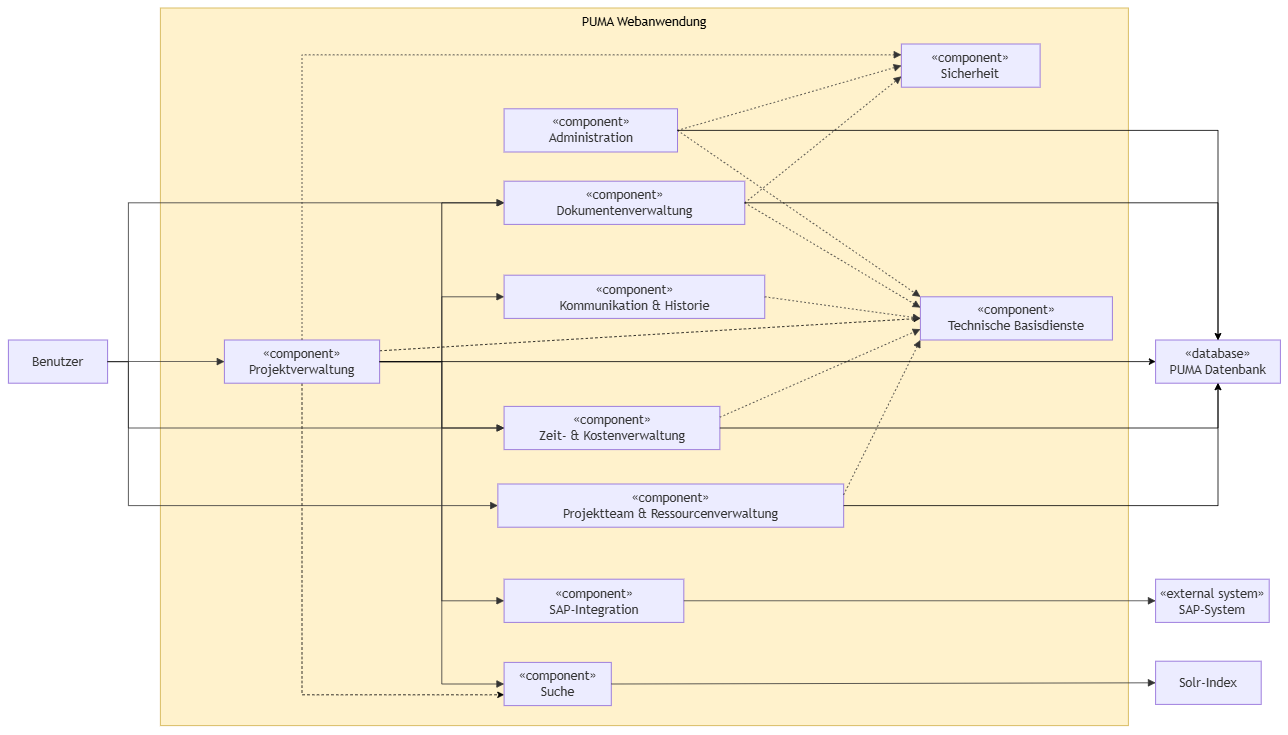
\includegraphics[width=1\textwidth]{assets/img/REALUMLFallPrax.png}}
    \caption{Fachliche und technische Struktur der Webanwendung Puma}
    \label{fig:uml_komponenten}
\end{figure}


\subsection{Beschreibung der Testszenarien}
\label{sec:testszenarien}

Dieses Unterkapitel beschreibt die getesteten Anwendungsszenarien systematisch und ordnet diese den jeweiligen Testklassen aus Selenium und den Testdateien aus Cypress zu.

\subsubsection{Szenario 1: Login}
Das Ziel dieses Tests ist es zu prüfen, ob sich ein Benutzer erfolgreich an der Puma-Webanwendung anmelden kann. Die Startbedingungen setzen voraus, dass Puma lokal über den Tomcat-Server auf Port \textbf{8082} erreichbar ist und ein gültiger Benutzer mit Benutzername und Passwort zur Verfügung steht.

Der Ablauf des Tests beginnt mit dem Öffnen der Login-Seite. Nach der Eingabe von Benutzername und Passwort wird der Login-Button betätigt. Anschließend wird geprüft, ob eine Weiterleitung auf die erwartete Zielseite erfolgt.

Das erwartete Ergebnis ist, dass der Benutzer erfolgreich angemeldet wird. Die Anwendung leitet auf die korrekte Folgeseite weiter, wobei dieser Redirect im Test validiert wird.

\textbf{Zuordnung der Testdateien:}
\begin{itemize}
    \item \textbf{Selenium:} \\ 
    \path{/ui-tests/src/test/java/ui/pumaTests/_login_Test/_01_PumaLoginTest.java}
    \item \textbf{Cypress:} \\ 
    \path{/my-springboot-app-e2e/cypress/e2e/Jumo Tests/Puma_login/01_login-ui.cy.js}
\end{itemize}


\subsubsection{Szenario 2: Neues Projekt bzw. neue Aktivität anlegen}
In diesem Szenario wird geprüft, ob ein neues Projekt bzw. eine neue Aktivität korrekt über die Benutzeroberfläche angelegt werden kann. Als Startbedingung muss der Benutzer erfolgreich angemeldet sein. Zudem muss die Anwendung lokal erreichbar sein und die benötigten Dropdown-Werte müssen im System zur Verfügung stehen.

Der Test navigiert zur Maske für die Projekt- bzw. Aktivitätsanlage. Dort wird das Stammblatt durch Eingabe der benötigten Projektdaten ausgefüllt und es werden relevante Werte in Dropdown-Feldern ausgewählt. Eine Besonderheit bilden hier Dropdowns mit \textbf{select2}, die dynamisch reagieren und daher gezielt im Code angesprochen werden müssen. Nach dem Ausfüllen wird das Formular gespeichert und die Systemrückmeldung geprüft.

Als erwartetes Ergebnis wird das Projekt oder die Aktivität erfolgreich angelegt. Die Anwendung zeigt eine korrekte Bestätigung oder Systemmeldung an, und die eingegebenen Daten sind anschließend im System vorhanden.

\textbf{Zuordnung der Testdateien:}
\begin{itemize}
    \item \textbf{Selenium:} \\ 
    \path{/ui-tests/src/test/java/ui/pumaTests/new_Activity/_02_NewActivityAnlegenTest.java} \\
    \path{/ui-tests/src/test/java/ui/pumaTests/new_Projekt/_02_NewProjektTest.java}
    \item \textbf{Cypress:} \\ 
    \path{/my-springboot-app-e2e/cypress/e2e/Jumo Tests/Puma_new_Activity(form Fill)/02_newActivity.cy.js} \\
    \path{/my-springboot-app-e2e/cypress/e2e/Jumo Tests/Puma_new_Projekt(Form_fill)/02_newProjekt.cy.js}
\end{itemize}


\subsubsection{Szenario 3: Aktivität bearbeiten}
Das Ziel des dritten Szenarios ist die Prüfung, ob eine bestehende Aktivität geöffnet, geändert, gespeichert und anschließend korrekt validiert werden kann. Die Startbedingungen erfordern, dass der Benutzer angemeldet ist, bereits eine bestehende Aktivität vorhanden ist und diese über die Benutzeroberfläche aufgerufen werden kann.

Der Ablauf sieht die Navigation zur bestehenden Aktivität sowie das Öffnen der Bearbeitungsansicht vor. Es folgt die Änderung definierter Werte, wie beispielsweise des Fortschritts oder des Datums. Nach dem Speichern der Änderungen wird die Aktivität erneut aufgerufen, um zu validieren, ob die Änderungen korrekt übernommen wurden.

Es wird erwartet, dass die Aktivität erfolgreich gespeichert wird und die geänderten Werte korrekt in der Oberfläche angezeigt werden. Die anschließende Kontrollprüfung muss die Bearbeitung bestätigen.

\textbf{Zuordnung der Testdateien:}
\begin{itemize}
    \item \textbf{Selenium:} \\ 
    \path{/ui-tests/src/test/java/ui/pumaTests/_edit_Data/_03_ControlEditedActivityTest.java} \\
    \path{/ui-tests/src/test/java/ui/pumaTests/_edit_Data/_03_EditActivityTest.java}
    
    \item \textbf{Cypress:} \\ 
    \path{/my-springboot-app-e2e/cypress/e2e/Jumo Tests/Puma_Edit_Data/03_controlEditedActivity.cy.js} \\
    \path{/my-springboot-app-e2e/cypress/e2e/Jumo Tests/Puma_Edit_Data/03_editActivity.cy.js}
\end{itemize}


\subsection{Setup und technische Integration}
\label{sec:setup}

Dieses Unterkapitel erläutert, wie Selenium und Cypress technisch in die bestehende Entwicklungsumgebung integriert wurden und welche spezifischen Herausforderungen dabei aufgetreten sind.

\subsubsection{Selenium}
Selenium wurde als Bibliothek in die bestehende Java-Umgebung integriert. Die Einbindung erfolgte unkompliziert über die \textbf{pom.xml} mit Maven. Da im Projekt ohnehin mit Java, Eclipse und Maven gearbeitet wird, passt das Framework sehr gut zur bestehenden Entwicklungsumgebung. Die Integration verlief weitgehend reibungslos. Ein anfängliches Kompatibilitätsproblem mit der im Unternehmen verwendeten älteren JDK-Version konnte umgangen werden.

Selenium ließ sich aufgrund der bestehenden Java- und Maven-Struktur gut in die vorhandene Entwicklungsumgebung integrieren.

\subsubsection{Cypress}
Im Gegensatz zur etablierten Java-basierten Integration von Selenium setzt Cypress eine Node.js- und npm-Umgebung voraus. Im vorliegenden Unternehmenskontext erwies sich diese technologische Anforderung als erste Hürde: Strikte Proxy- und Sicherheitsrichtlinien blockierten die reguläre Paketinstallation über npm, weshalb eine dedizierte IT-Freigabe zwingend erforderlich war.

Zwar kann eine lokale Installation über ein ZIP-Archiv als kurzfristiger Workaround dienen, dieser Ansatz wurde jedoch verworfen. Er eignet sich nicht für wiederholbare, skalierbare Continuous-Integration-Prozesse (CI) und erschwert die saubere Versionsverwaltung. Folglich bleibt der initiale Einrichtungsaufwand für Cypress -- trotz der grundsätzlichen Lösbarkeit durch administrative Freigabeprozesse -- im direkten Vergleich zu Selenium organisatorisch und technisch umständlicher.

\subsection{Syntax- und Architekturvergleich}
\label{sec:syntaxvergleich}

Die Frameworks Selenium und Cypress unterscheiden sich grundlegend in Bezug auf Architektur, Syntax, Wartbarkeit und Synchronisation.

\subsubsection{Architektur}
Selenium wird als Bibliothek in die bestehende Java/JUnit-Umgebung integriert \cite{spillner2024basiswissen}. Es arbeitet als Bestandteil des vorhandenen Maven-Projekts, wodurch die Testautomatisierung eng mit der bestehenden Backend- bzw. Java-Struktur verbunden ist. Cypress hingegen ist ein eigenständiges Tooling auf Basis von Node.js und bringt eine eigene Testumgebung mit. Es läuft nicht als Java-Bibliothek, sondern agiert als separates End-to-End-Testframework.

Zusammenfassend: Selenium erweitert die vorhandene Java-Testumgebung, während Cypress eine eigenständige Testplattform auf Basis von Node.js bereitstellt.

\subsubsection{Ausdrucksstärke der Syntax}
Cypress zeichnet sich durch eine Syntax aus, die näher an natürlicher Sprache ist. Befehle lassen sich über das Konzept des Chainings gut lesbar aneinanderreihen. Durch Befehle wie \textbf{cy.get(...).type(...)} entsteht eine kompakte und gut lesbare Testbeschreibung.

Selenium ist hingegen technischer und stärker objektorientiert geprägt. Bevor eine Interaktion stattfinden kann, müssen DOM-Elemente in der Regel explizit als \textbf{WebElement} gespeichert werden. Die tatsächliche Interaktion erfolgt erst im nächsten Schritt über Methoden wie \textbf{clear()} und \textbf{sendKeys()}.

\subsubsection{Wartbarkeit}
Bei der Nutzung von Selenium entstehen ohne strukturierende Maßnahmen schnell Wiederholungen im Quellcode. Um Redundanzen zu vermeiden, sind Hilfsmethoden oder die Anwendung des Page-Object-Patterns als notwendige Strukturierungsmaßnahmen unerlässlich \cite{Liggesmeyer2009}.

Cypress ermöglicht durch Chaining und implizite Mechanismen häufig kompakteren Code. Gerade einfache Testabläufe wirken dadurch übersichtlicher, auch wenn bei steigender Projektkomplexität ebenso in Cypress eine strukturierte Testorganisation erforderlich sein kann.

\subsubsection{Synchronisation}
Ein zentraler Unterschied liegt in der Handhabung dynamischer Ladezeiten. In Selenium müssen dynamische Elemente häufig explizit mit Anweisungen wie \textbf{wait.until(...)} behandelt werden. Die Sichtbarkeit oder Klickbarkeit muss aktiv geprüft werden, was den Code umfangreicher macht.

Cypress verfügt über integrierte Auto-Waits. Viele Wartebedingungen sind bereits in den Basisbefehlen wie \textbf{cy.get()}, \textbf{type()} oder \textbf{click()} enthalten, wodurch sich der manuelle Synchronisationsaufwand maßgeblich verringert.

Der wesentliche Unterschied liegt darin, dass Selenium Wartebedingungen häufig explizit formuliert, während Cypress viele Synchronisationsaufgaben automatisch übernimmt.


\subsection{Code-Gegenüberstellung: Projektanlage}
\label{sec:code_gegenueberstellung}

Anhand eines ausgewählten Codebeispiels wird im Folgenden der strukturelle Aufbau beider Frameworks bei typischen UI-Interaktionen gegenübergestellt. Der Schwerpunkt dieses Vergleichs liegt auf dem Befüllen von Formularfeldern, konkret dem Setzen des Projektnamens und des Enddatums bei der Projektanlage.

% PLATZHALTER: Screenshot Selenium
\begin{figure}[H]
    \centering
    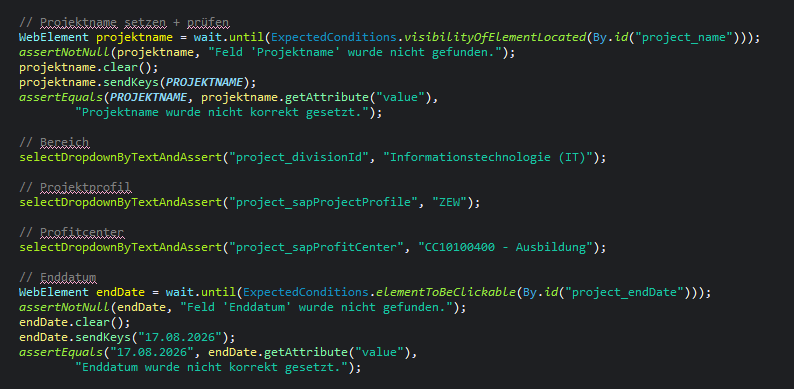
\includegraphics[width=1\textwidth]{assets/img/SeleniumCodeVs.png}
    \caption{Ausführung der Projektanlage mittels Selenium}
    \label{fig:selenium_projektanlage}
\end{figure}

Wie im Quellcode erkennbar, wird für jedes relevante Element in Selenium zunächst ein explizites Warten (Wait) definiert. Beim Feld \texttt{project\_name} wird auf die Sichtbarkeit gewartet, beim Feld \texttt{project\_endDate} auf die Klickbarkeit. Erst danach können die Felder geleert und mit den Testdaten befüllt werden. Dies macht den Code zwar robust gegenüber dynamischen Ladezeiten, erhöht jedoch die Zeilenanzahl und verleiht dem Test einen stark technischen Charakter.

% PLATZHALTER: Screenshot Cypress
\begin{figure}[H]
    \centering
    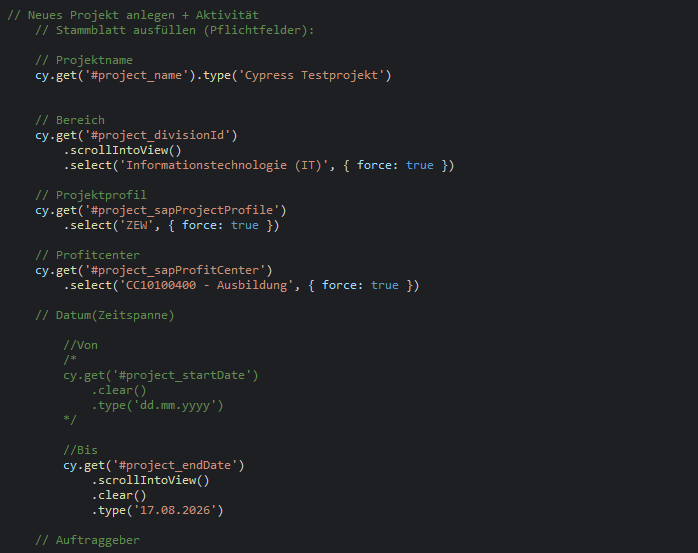
\includegraphics[width=1\textwidth]{assets/img/CypressCodeVs.png}
    \caption{Ausführung der Projektanlage im Cypress Test Runner}
    \label{fig:cypress_projektanlage}
\end{figure}

Cypress nutzt im Gegensatz dazu, wie in Quellcode \ref{lst:cypress_form} dargestellt, die Anweisung \texttt{cy.get()} zur Auswahl des Elements. Notwendige Wartebedingungen sind in den Cypress-Standardbefehlen bereits implizit integriert, sodass die Aktionen direkt verkettet (Chaining) werden können. Für das Datumsfeld wird zusätzlich \texttt{scrollIntoView()} verwendet, um sicherzustellen, dass sich das Element im sichtbaren Viewport befindet. 

Aus dieser Gegenüberstellung lassen sich folgende Bewertungsaspekte für die Nutzwertanalyse ableiten:
\begin{enumerate}
    \item \textbf{Synchronisation:} Selenium erfordert bei dynamischen Oberflächen die manuelle Definition expliziter Waits. Cypress kapselt diese Wartebedingungen in seinen Standardbefehlen.
    \item \textbf{Codeumfang:} Selenium benötigt mehr Programmzeilen, da Wartebedingungen und Elementvariablen separiert werden. Cypress erreicht durch das Chaining eine kompaktere Darstellung.
    \item \textbf{Lesbarkeit:} Der Selenium-Code ist stark technisch strukturiert. Die Cypress-Syntax liest sich hingegen eher wie eine direkte funktionale Beschreibung der Anwenderaktion.
    \item \textbf{Wartbarkeit:} Während Cypress einfache UI-Abläufe nativ kompakt hält, erfordert Selenium bei wachsendem Testumfang zwingend den Einsatz von Hilfsmethoden oder Architekturmustern (wie dem Page Object Model), um die Wartbarkeit sicherzustellen.
\end{enumerate}

Zusammenfassend zeigt der Vergleich, dass Selenium eine sehr feingranulare Steuerung der Synchronisation ermöglicht, was jedoch den Code-Overhead erhöht. Cypress bietet insbesondere bei formularbasierten Interaktionen eine lesbarere und kompaktere Syntax, was die Einarbeitung und Pflege der Tests erleichtert.